%% This file was auto-generated by IPython.
%% Conversion from the original notebook file:
%% kmeans.ipynb
%%
\documentclass[11pt,english,fleqn]{article}

%% This is the automatic preamble used by IPython.  Note that it does *not*
%% include a documentclass declaration, that is added at runtime to the overall
%% document.

\usepackage{amsmath}
\usepackage{amssymb}
\usepackage{graphicx}
\usepackage{ucs}
\usepackage[utf8x]{inputenc}

% needed for markdown enumerations to work
\usepackage{enumerate}

% Slightly bigger margins than the latex defaults
\usepackage{geometry}
\geometry{verbose,tmargin=3cm,bmargin=3cm,lmargin=2.5cm,rmargin=2.5cm}

% Define a few colors for use in code, links and cell shading
\usepackage{color}
\definecolor{orange}{cmyk}{0,0.4,0.8,0.2}
\definecolor{darkorange}{rgb}{.71,0.21,0.01}
\definecolor{darkgreen}{rgb}{.12,.54,.11}
\definecolor{myteal}{rgb}{.26, .44, .56}
\definecolor{gray}{gray}{0.45}
\definecolor{lightgray}{gray}{.95}
\definecolor{mediumgray}{gray}{.8}
\definecolor{inputbackground}{rgb}{.95, .95, .85}
\definecolor{outputbackground}{rgb}{.95, .95, .95}
\definecolor{traceback}{rgb}{1, .95, .95}

% Framed environments for code cells (inputs, outputs, errors, ...).  The
% various uses of \unskip (or not) at the end were fine-tuned by hand, so don't
% randomly change them unless you're sure of the effect it will have.
\usepackage{framed}

% remove extraneous vertical space in boxes
\setlength\fboxsep{0pt}

% codecell is the whole input+output set of blocks that a Code cell can
% generate.

% TODO: unfortunately, it seems that using a framed codecell environment breaks
% the ability of the frames inside of it to be broken across pages.  This
% causes at least the problem of having lots of empty space at the bottom of
% pages as new frames are moved to the next page, and if a single frame is too
% long to fit on a page, will completely stop latex from compiling the
% document.  So unless we figure out a solution to this, we'll have to instead
% leave the codecell env. as empty.  I'm keeping the original codecell
% definition here (a thin vertical bar) for reference, in case we find a
% solution to the page break issue.

%% \newenvironment{codecell}{%
%%     \def\FrameCommand{\color{mediumgray} \vrule width 1pt \hspace{5pt}}%
%%    \MakeFramed{\vspace{-0.5em}}}
%%  {\unskip\endMakeFramed}

% For now, make this a no-op...
\newenvironment{codecell}{}

 \newenvironment{codeinput}{%
   \def\FrameCommand{\colorbox{inputbackground}}%
   \MakeFramed{\advance\hsize-\width \FrameRestore}}
 {\unskip\endMakeFramed}

\newenvironment{codeoutput}{%
   \def\FrameCommand{\colorbox{outputbackground}}%
   \vspace{-1.4em}
   \MakeFramed{\advance\hsize-\width \FrameRestore}}
 {\unskip\medskip\endMakeFramed}

\newenvironment{traceback}{%
   \def\FrameCommand{\colorbox{traceback}}%
   \MakeFramed{\advance\hsize-\width \FrameRestore}}
 {\endMakeFramed}

% Use and configure listings package for nicely formatted code
\usepackage{listingsutf8}
\lstset{
  language=python,
  inputencoding=utf8x,
  extendedchars=\true,
  aboveskip=\smallskipamount,
  belowskip=\smallskipamount,
  xleftmargin=2mm,
  breaklines=true,
  basicstyle=\small \ttfamily,
  showstringspaces=false,
  keywordstyle=\color{blue}\bfseries,
  commentstyle=\color{myteal},
  stringstyle=\color{darkgreen},
  identifierstyle=\color{darkorange},
  columns=fullflexible,  % tighter character kerning, like verb
}

% The hyperref package gives us a pdf with properly built
% internal navigation ('pdf bookmarks' for the table of contents,
% internal cross-reference links, web links for URLs, etc.)
\usepackage{hyperref}
\hypersetup{
  breaklinks=true,  % so long urls are correctly broken across lines
  colorlinks=true,
  urlcolor=blue,
  linkcolor=darkorange,
  citecolor=darkgreen,
  }

% hardcode size of all verbatim environments to be a bit smaller
\makeatletter 
\g@addto@macro\@verbatim\small\topsep=0.5em\partopsep=0pt
\makeatother 

% Prevent overflowing lines due to urls and other hard-to-break entities.
\sloppy

\setlength{\mathindent}{0pt}
\setlength{\parindent}{0pt}
\setlength{\parskip}{8pt}
\begin{document}

\subsection{Hadoop ve KMeans}

Some text goes here

\begin{codecell}
\begin{codeinput}
\begin{lstlisting}
from pandas import *
df = read_csv("synthetic.txt",names=['a','b'],sep="   ")
scatter(df['a'],df['b'])

\end{lstlisting}
\end{codeinput}
\begin{codeoutput}
\begin{verbatim}
<matplotlib.collections.PathCollection at 0xa6f320c>
\end{verbatim}
\begin{center}
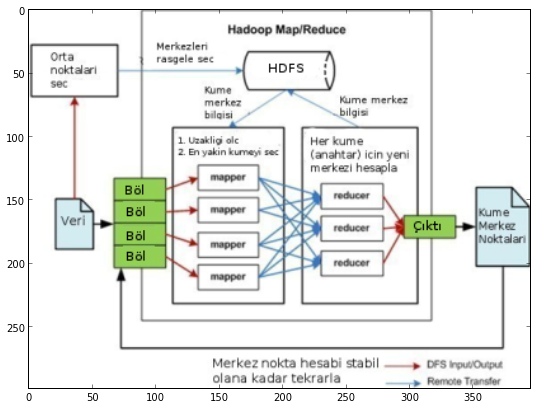
\includegraphics[width=0.7\textwidth]{kmeans_files/kmeans_fig_00.png}
\par
\end{center}
\end{codeoutput}
\end{codecell}
\begin{codecell}
\begin{codeinput}
\begin{lstlisting}
!ssh localhost -l hduser /home/hduser/Downloads/hadoop*/bin/stop-all.sh
!ssh localhost -l hduser /home/hduser/Downloads/hadoop*/bin/start-all.sh

\end{lstlisting}
\end{codeinput}
\begin{codeoutput}
\begin{verbatim}
no jobtracker to stop
\end{verbatim}
\begin{verbatim}
localhost: no tasktracker to stop
\end{verbatim}
\begin{verbatim}
no namenode to stop
\end{verbatim}
\begin{verbatim}
localhost: no datanode to stop
\end{verbatim}
\begin{verbatim}
localhost: no secondarynamenode to stop
\end{verbatim}
\begin{verbatim}
starting namenode, logging to /home/hduser/Downloads/hadoop-1.0.4/libexec/../logs/hadoop-hduser-namenode-burak-Aspire-S3.out
\end{verbatim}
\begin{verbatim}
localhost: starting datanode, logging to /home/hduser/Downloads/hadoop-1.0.4/libexec/../logs/hadoop-hduser-datanode-burak-Aspire-S3.out
\end{verbatim}
\begin{verbatim}
localhost: starting secondarynamenode, logging to /home/hduser/Downloads/hadoop-1.0.4/libexec/../logs/hadoop-hduser-secondarynamenode-burak-Aspire-S3.out
\end{verbatim}
\begin{verbatim}
starting jobtracker, logging to /home/hduser/Downloads/hadoop-1.0.4/libexec/../logs/hadoop-hduser-jobtracker-burak-Aspire-S3.out
\end{verbatim}
\begin{verbatim}
localhost: starting tasktracker, logging to /home/hduser/Downloads/hadoop-1.0.4/libexec/../logs/hadoop-hduser-tasktracker-burak-Aspire-S3.out
\end{verbatim}
\end{codeoutput}
\end{codecell}
\begin{codecell}
\begin{codeinput}
\begin{lstlisting}
!ssh localhost -l hduser /home/hduser/Downloads/hadoop*/bin/hadoop dfs -mkdir /tmp/
\end{lstlisting}
\end{codeinput}
\end{codecell}
\begin{codecell}
\begin{codeinput}
\begin{lstlisting}
!ssh localhost -l hduser /home/hduser/Downloads/hadoop*/bin/hadoop dfs -ls /
\end{lstlisting}
\end{codeinput}
\begin{codeoutput}
\begin{verbatim}
Found 3 items
drwxr-xr-x   - hduser supergroup          0 2013-02-25 17:23 /app
drwxr-xr-x   - hduser supergroup          0 2013-02-26 12:49 /tmp
drwxr-xr-x   - hduser supergroup          0 2013-02-26 11:45 /user
\end{verbatim}
\end{codeoutput}
\end{codecell}
\begin{codecell}
\begin{codeinput}
\begin{lstlisting}
!ssh localhost -l hduser /home/hduser/Downloads/hadoop*/bin/hadoop dfs -copyFromLocal $HOME/Documents/classnotes/stat/stat_hadoop_kmeans/synthetic.txt /user/hduser
\end{lstlisting}
\end{codeinput}
\begin{codeoutput}
\begin{verbatim}
copyFromLocal: Target /user/hduser/synthetic.txt already exists
\end{verbatim}
\end{codeoutput}
\end{codecell}
\begin{codecell}
\begin{codeinput}
\begin{lstlisting}
!cp mapper.py /tmp/
!chmod a+r /tmp/mapper.py
!chmod a+x /tmp/mapper.py
!ssh localhost -l hduser /home/hduser/Downloads/hadoop*/bin/hadoop dfs -rmr /user/hduser/output


\end{lstlisting}
\end{codeinput}
\begin{codeoutput}
\begin{verbatim}
Deleted hdfs://localhost:54310/user/hduser/output
\end{verbatim}
\begin{verbatim}
packageJobJar: [/app/hadoop/tmp/hadoop-unjar4901234381683438453/] [] /tmp/streamjob8733192798849770485.jar tmpDir=null
\end{verbatim}
\begin{verbatim}
13/02/27 01:00:48 INFO util.NativeCodeLoader: Loaded the native-hadoop library
13/02/27 01:00:48 WARN snappy.LoadSnappy: Snappy native library not loaded
13/02/27 01:00:48 INFO mapred.FileInputFormat: Total input paths to process : 1
\end{verbatim}
\begin{verbatim}
13/02/27 01:00:48 INFO streaming.StreamJob: getLocalDirs(): [/app/hadoop/tmp/mapred/local]
13/02/27 01:00:48 INFO streaming.StreamJob: Running job: job_201302270038_0001
13/02/27 01:00:48 INFO streaming.StreamJob: To kill this job, run:
13/02/27 01:00:48 INFO streaming.StreamJob: /home/hduser/Downloads/hadoop-1.0.4/libexec/../bin/hadoop job  -Dmapred.job.tracker=localhost:54311 -kill job_201302270038_0001
13/02/27 01:00:48 INFO streaming.StreamJob: Tracking URL: http://localhost:50030/jobdetails.jsp?jobid=job_201302270038_0001
\end{verbatim}
\begin{verbatim}
13/02/27 01:00:49 INFO streaming.StreamJob:  map 0%  reduce 0%
\end{verbatim}
\begin{verbatim}
13/02/27 01:01:37 INFO streaming.StreamJob:  map 100%  reduce 100%
13/02/27 01:01:37 INFO streaming.StreamJob: To kill this job, run:
13/02/27 01:01:37 INFO streaming.StreamJob: /home/hduser/Downloads/hadoop-1.0.4/libexec/../bin/hadoop job  -Dmapred.job.tracker=localhost:54311 -kill job_201302270038_0001
13/02/27 01:01:37 INFO streaming.StreamJob: Tracking URL: http://localhost:50030/jobdetails.jsp?jobid=job_201302270038_0001
13/02/27 01:01:37 ERROR streaming.StreamJob: Job not successful. Error: # of failed Map Tasks exceeded allowed limit. FailedCount: 1. LastFailedTask: task_201302270038_0001_m_000000
13/02/27 01:01:37 INFO streaming.StreamJob: killJob...
Streaming Command Failed!
\end{verbatim}
\end{codeoutput}
\end{codecell}
\begin{codecell}
\begin{codeinput}
\begin{lstlisting}
print open("mapper.py").read()
\end{lstlisting}
\end{codeinput}
\begin{codeoutput}
\begin{verbatim}
#!/usr/bin/python
import os,sys,itertools
import numpy as np
from numpy import linalg as la
os.environ['MPLCONFIGDIR']='/tmp' 
import pandas as pd

centers = pd.read_csv("/tmp/centers.csv",header=None,sep=",")
print centers[:4]

def dist(vect,x):
    return np.fromiter(itertools.imap(np.linalg.norm, vect-x),dtype=np.float)

def closest(x):
    d = dist(np.array(centers)[:,1:3],np.array(x))
    return np.argmin(d)

df = pd.read_csv(sys.stdin,header=None,sep="   ")
df['closest'] = df.apply(closest,axis=1)
print df[:20]
\end{verbatim}
\end{codeoutput}
\end{codecell}
\begin{codecell}
\begin{codeinput}
\begin{lstlisting}
import os,sys,itertools
from numpy import linalg as la
import pandas as pd
k = 10
df = read_csv("synthetic.txt",names=['a','b'],sep="   ")
centers = df.take(np.random.permutation(len(df))[:k])
centers.to_csv("/tmp/centers.csv",header=None)

os.system("cp mapper.py /tmp/")
os.system("chmod a+r /tmp/mapper.py")
os.system("chmod a+x /tmp/mapper.py")

os.system("ssh localhost -l hduser /home/hduser/Downloads/hadoop*/bin/hadoop dfs -rm /user/hduser/centers.csv")
os.system("ssh localhost -l hduser /home/hduser/Downloads/hadoop*/bin/hadoop dfs -copyFromLocal /tmp/centers.csv /user/hduser")
os.system("ssh localhost -l hduser /home/hduser/Downloads/hadoop*/bin/hadoop dfs -cat /user/hduser/centers.csv")

centers = pd.read_csv("/tmp/centers.csv",header=None,sep=",")
print centers[:4]

os.system("ssh localhost -l hduser /home/hduser/Downloads/hadoop*/bin/hadoop dfs -rmr /user/hduser/output")
os.system("ssh localhost -l hduser /home/hduser/Downloads/hadoop*/bin/hadoop  jar /home/hduser/Downloads/hadoop*/contrib/streaming/hadoop-*streaming*.jar -input patent/apat63_99_sampled.txt  -output output  -mapper /tmp/mapper.py -numReduceTasks 0 ")

\end{lstlisting}
\end{codeinput}
\begin{codeoutput}
\begin{verbatim}
0      1      2
0  2145  28810  55914
1  2687   9657  50553
2  2091  30265  59751
3  1830  37166  58232
\end{verbatim}
\begin{verbatim}
1024
\end{verbatim}
\end{codeoutput}
\end{codecell}
\begin{codecell}
\begin{codeinput}
\begin{lstlisting}
xfrom IPython.core.display import HTML
def css_styling():
    styles = open("../../custom.css", "r").read()
    return HTML(styles)
css_styling()
\end{lstlisting}
\end{codeinput}
\begin{codeoutput}
\begin{verbatim}
<IPython.core.display.HTML at 0xa34402c>
\end{verbatim}
\end{codeoutput}
\end{codecell}

\end{document}
